% ============================================================
% Relatório EEL891 --- Aprendizado de Máquina --- UFRJ
% Compilar no Overleaf com pdflatex
% Upload: este .tex + ufrj_logo_1.jpeg, ufrj_logo_2.png
%         + eda_visualizacoes.png, feature_importance.png
% ============================================================
\documentclass[12pt, a4paper]{article}

\usepackage[utf8]{inputenc}
\usepackage[T1]{fontenc}
\usepackage[brazil]{babel}
\usepackage{lmodern}
\usepackage[top=2.5cm, bottom=2.5cm, left=3cm, right=2.5cm, footskip=1.25cm]{geometry}
\usepackage{setspace}
\onehalfspacing
\setlength{\parindent}{1.25cm}
\setlength{\parskip}{0pt}

\usepackage{fancyhdr}
\pagestyle{fancy}
\fancyhf{}
\fancyhead[L]{\small Trabalho 1: Inadimplência de Crédito}
\fancyhead[R]{\small Aprendizado de Máquina (EEL891)}
\fancyfoot[C]{\thepage}
\renewcommand{\headrulewidth}{0.4pt}

\usepackage{graphicx}
\usepackage{float}
\usepackage{caption}
\captionsetup{font=small, labelfont=bf, justification=centering}

\usepackage{booktabs}
\usepackage{tabularx}
\usepackage{array}
\usepackage[table,xcdraw]{xcolor}
\definecolor{headerblue}{RGB}{31,78,121}
\definecolor{rowalt}{RGB}{238,243,248}

\usepackage{listings}
\definecolor{codebg}{RGB}{245,245,245}
\definecolor{codecomment}{RGB}{100,100,100}
\definecolor{codekey}{RGB}{31,78,121}

\lstdefinestyle{pythonstyle}{
  backgroundcolor=\color{codebg},
  basicstyle=\ttfamily\footnotesize,
  keywordstyle=\color{codekey}\bfseries,
  commentstyle=\color{codecomment}\itshape,
  language=Python, frame=single, framerule=0.4pt,
  rulecolor=\color{gray!40}, breaklines=true,
  numbers=left, numberstyle=\tiny\color{gray},
  numbersep=8pt, showstringspaces=false,
  tabsize=2, xleftmargin=1em,
  literate={ã}{{\~{a}}}1 {õ}{{\~{o}}}1 {ç}{{\c{c}}}1
           {á}{{\'a}}1  {é}{{\'e}}1   {í}{{\'i}}1
           {ó}{{\'o}}1  {ú}{{\'u}}1   {â}{{\^a}}1
           {ê}{{\^e}}1  {à}{{\`a}}1
}

\usepackage[colorlinks=true, linkcolor=headerblue, urlcolor=headerblue]{hyperref}
\usepackage{amsmath, amssymb}
\usepackage{enumitem}
\usepackage{titlesec}

\titleformat{\section}{\large\bfseries\color{headerblue}}{\thesection}{1em}{}
\titleformat{\subsection}{\normalsize\bfseries\color{headerblue!80}}{\thesubsection}{1em}{}
\titleformat{\subsubsection}{\normalsize\bfseries\color{headerblue!70}}{\thesubsubsection}{1em}{}

\newcommand{\code}[1]{\texttt{#1}}

\begin{document}
\pagenumbering{gobble}

% ── CAPA ─────────────────────────────────────────────────────
\begin{titlepage}
  \centering
  \begin{minipage}{0.35\textwidth}
    \centering
    \includegraphics[height=3.2cm]{ufrj_logo_1.jpeg}
  \end{minipage}
  \hfill
  \begin{minipage}{0.58\textwidth}
    \centering
    \includegraphics[height=3.2cm]{ufrj_logo_2.png}
  \end{minipage}

  \vspace{3.0cm}
  {\LARGE\bfseries EEL891 --- Introdução ao Aprendizado de Máquina\\[0.6em]}
  {\Huge\bfseries\color{headerblue} Trabalho 1\\[0.4em]}
  {\Large\bfseries\color{headerblue} Classificação de Inadimplência de Crédito\\[0.8em]}
  \vspace{0.4cm}
  {\large Classificador binário para apoio à decisão}

  \vspace{3.0cm}
  \begin{tabular}{rl}
    \textbf{Aluno:}       & Luiz Felipe Píccoli Cavalini \\[0.5em]
    \textbf{Ferramentas:} & Python 3.12 (\code{scikit-learn}, \code{LightGBM}, \\
                          & \code{XGBoost}, \code{CatBoost}, \code{Optuna}) \\
  \end{tabular}
  \vfill
  {\large Rio de Janeiro, Julho de 2026}
\end{titlepage}

\pagenumbering{roman}
\pagestyle{plain}
\begingroup
  \setlength{\parskip}{0pt}
  \renewcommand{\baselinestretch}{0.95}\normalfont
  \tableofcontents
\endgroup
\newpage
\pagenumbering{arabic}
\pagestyle{fancy}

\section{Introdução}

O presente trabalho consiste na construção de um classificador binário para apoio à decisão de aprovação de crédito. A partir de dados históricos de 20.000 solicitações de crédito, acompanhadas do desfecho (adimplência ou inadimplência), o objetivo é predizer o comportamento de 5.000 novas solicitações cujos desfechos são desconhecidos.

A métrica de avaliação é a \textbf{acurácia}, e as previsões são submetidas na plataforma Kaggle, que compara automaticamente com o gabarito oculto.

O pipeline adotado segue as etapas clássicas: análise exploratória, pré-processamento, engenharia de \textit{features}, modelagem com múltiplos algoritmos, otimização de hiperparâmetros e construção de \textit{ensembles}. As ferramentas utilizadas foram Python 3.12 com \code{pandas}~\cite{ref:pandas}, \code{scikit-learn}~\cite{ref:sklearn}, \code{LightGBM}~\cite{ref:lgbm}, \code{XGBoost}~\cite{ref:xgb}, \code{CatBoost}~\cite{ref:catboost} e \code{Optuna}~\cite{ref:optuna}.

\section{Análise Exploratória dos Dados}

\subsection{Estrutura e distribuição do \textit{target}}

O conjunto de treinamento contém 20.000 amostras e 41 colunas. A variável-alvo \code{inadimplente} é \textbf{perfeitamente balanceada}: 10.000 bons pagadores e 10.000 inadimplentes (50\%/50\%). Isso dispensa técnicas de balanceamento como SMOTE ou ajuste de \code{class\_weight}.

\subsection{Valores ausentes}

Seis colunas apresentam valores nulos. As mais afetadas são \code{grau\_instrucao\_companheiro} (64,3\%) e \code{profissao\_companheiro} (57,6\%), cujos altos percentuais indicam provável ausência de companheiro --- o que motivou a criação de uma \textit{feature} binária \code{tem\_companheiro}.

\subsection{Colunas descartadas}

Quatro colunas foram removidas: \code{grau\_instrucao} (100\% zeros), \code{possui\_telefone\_celular} (100\% ``N''), \code{qtde\_contas\_bancarias\_especiais} (idêntica a outra coluna) e \code{local\_onde\_\\trabalha} (idêntica a \code{local\_onde\_reside} em 100\% dos registros).

\subsection{Correlações e visualizações}

As correlações lineares com o \textit{target} são todas muito fracas (máximo $|r| = 0{,}12$ para \code{idade}), indicando que modelos lineares teriam desempenho limitado e que modelos não-lineares baseados em árvores~\cite{ref:friedman, ref:breiman} seriam mais adequados.

A Figura~\ref{fig:eda} apresenta a distribuição das variáveis mais relevantes, segmentadas por classe. Observa-se que nenhuma variável isolada separa bem as classes, confirmando a necessidade de combinações não-lineares.

\begin{figure}[H]
  \centering
  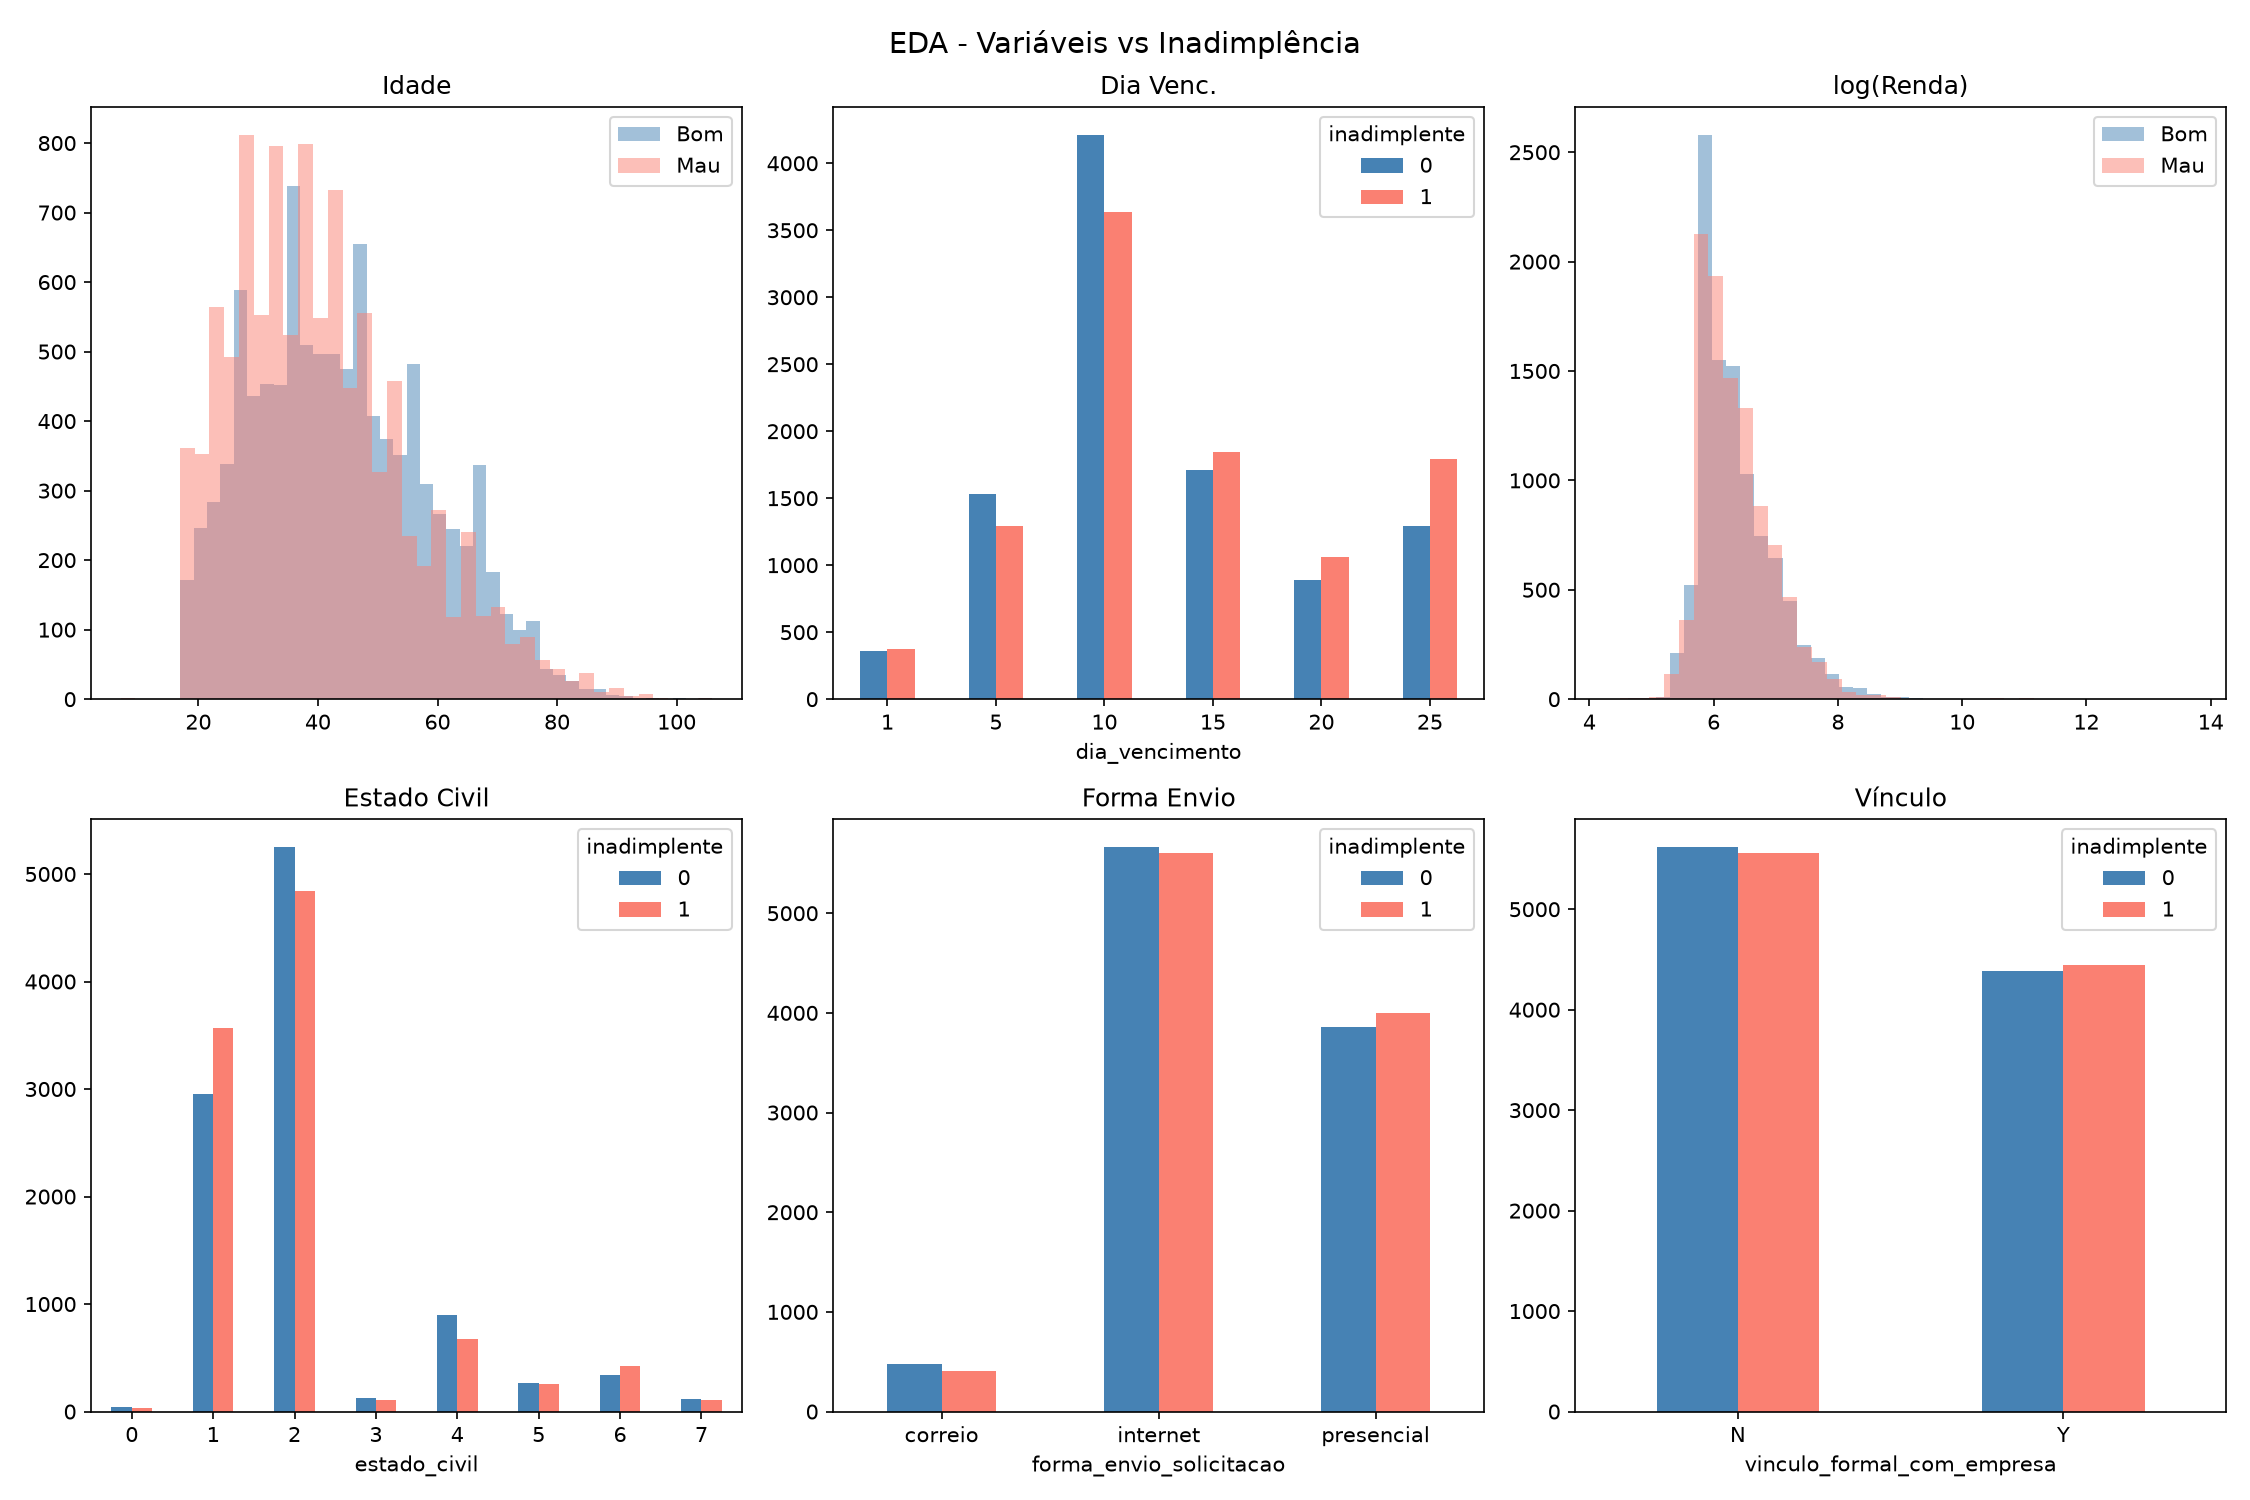
\includegraphics[width=1.0\textwidth]{eda_visualizacoes.png}
  \caption{Distribuição das principais variáveis por classe (azul = bom pagador, vermelho = inadimplente).}
  \label{fig:eda}
\end{figure}

\section{Pré-processamento}

\subsection{Variáveis textuais}

Valores em branco e códigos inválidos (``XX'') foram substituídos por categorias explícitas. As colunas Y/N foram convertidas para 0/1.

\subsection{Imputação de nulos}

A estratégia variou conforme o tipo: mediana para \code{meses\_na\_residencia}, moda para \code{tipo\_residencia}, e valor sentinela $-1$ para \code{profissao}, \code{ocupacao} e as variáveis de companheiro (indicando ``não informado'').

\section{Engenharia de \textit{Features}}

Foram criadas 14 novas variáveis a partir dos atributos originais. A escolha de cada uma foi guiada pelo conhecimento do domínio de crédito e pela análise exploratória:

\begin{itemize}[leftmargin=2em, nosep]
  \item \textbf{Financeiras:} \code{renda\_total} (soma de renda regular e extra, capturando a capacidade de pagamento completa), \code{tem\_renda\_extra} (flag: fontes adicionais de renda indicam maior estabilidade), \code{razao\_patrimonio\_renda} (patrimônio dividido pela renda --- um patrimônio alto relativo à renda sugere solidez financeira acumulada).
  \item \textbf{Cartões:} \code{qtde\_cartoes} e \code{tem\_algum\_cartao} --- a posse de cartões indica acesso prévio a crédito e histórico no sistema financeiro.
  \item \textbf{Geográficas:} \code{reside\_mesmo\_estado} e \code{trabalha\_mesmo\_estado} --- estabilidade geográfica pode correlacionar com estabilidade financeira.
  \item \textbf{Contato:} \code{qtde\_telefones} --- mais pontos de contato sugerem maior rastreabilidade do solicitante.
  \item \textbf{Transformações:} \code{faixa\_etaria} (discretização da idade em 6 faixas, permitindo ao modelo capturar efeitos não-monotônicos), \code{log\_renda}, \code{log\_patrimonio} e \code{log\_renda\_total} (reduzir a assimetria causada por \textit{outliers} extremos, como rendas de até R\$ 959.000).
  \item \textbf{Interações:} \code{idade\_x\_renda} (uma pessoa jovem com renda alta tem perfil diferente de uma idosa com a mesma renda --- a interação captura esse efeito) e \code{vinculo\_x\_renda} (renda com vínculo formal tem significado diferente de renda informal de mesmo valor).
\end{itemize}

\section{Codificação de Variáveis Categóricas}

\subsection{Label Encoding}

Aplicado a \code{sexo} (3 categorias) e \code{forma\_envio\_solicitacao} (5 categorias).

\subsection{Target Encoding}

Para variáveis de alta cardinalidade (\code{estado\_onde\_nasceu}, \code{estado\_onde\_reside}, \code{estado\_\\onde\_trabalha}, \code{codigo\_area\_telefone\_residencial}, \code{codigo\_area\_telefone\_trabalho}), cada categoria foi substituída pela proporção média de inadimplentes, calculada \textbf{exclusivamente no conjunto de treinamento}, seguindo a técnica descrita por Micci-Barreca~\cite{ref:micci}.

\subsubsection{Abordagens testadas e descartadas}

Durante o desenvolvimento, foram testadas variações de encoding:

\begin{itemize}[leftmargin=2em]
  \item \textbf{Target encoding expandido:} estender o \textit{target encoding} para todas as variáveis categóricas numéricas (\code{profissao}, \code{ocupacao}, \code{dia\_vencimento}, etc.). A validação cruzada indicou um ganho expressivo (0,604 $\to$ 0,636), porém ao submeter ao Kaggle a acurácia \textbf{caiu para 0,589}. A causa foi identificada como \textbf{\textit{data leakage}}: o encoding é calculado com informação do \textit{target} no treino inteiro, incluindo os folds de validação, inflando artificialmente a CV.
  \item \textbf{Target encoding out-of-fold:} tentou-se corrigir o \textit{leakage} calculando o encoding em cada fold separadamente. A CV ficou mais honesta (0,609), mas o Kaggle ainda retornou 0,594 --- confirmando que essas variáveis, com muitas categorias raras, não se beneficiam dessa técnica.
  \item \textbf{Encoding ordinal puro} (sem \textit{target encoding}): piorou para 0,587, confirmando a utilidade do \textit{target encoding} para as 5 variáveis de estado e telefone.
\end{itemize}

\textbf{Conclusão:} o \textit{target encoding} foi mantido apenas para as 5 variáveis de alta cardinalidade textuais, que demonstraram consistência entre CV e Kaggle.

\section{Modelagem}

\subsection{Validação cruzada}

Todos os modelos foram avaliados com \textbf{5-Fold Stratified Cross-Validation}, mantendo a proporção 50/50 do \textit{target} em cada fold.

\subsection{Modelos base}

A Tabela~\ref{tab:baselines} apresenta os resultados dos modelos com hiperparâmetros padrão.

\begin{table}[H]
  \centering
  \caption{Acurácia CV dos modelos base}
  \label{tab:baselines}
  \small\rowcolors{2}{rowalt}{white}
  \begin{tabular}{lcc}
    \toprule
    \rowcolor{headerblue}
    \color{white}\textbf{Modelo} & \color{white}\textbf{Acurácia CV} & \color{white}\textbf{Desvio} \\
    \midrule
    Regressão Logística     & 0,5638 & 0,0075 \\
    Random Forest~\cite{ref:breiman}  & 0,6006 & 0,0090 \\
    LightGBM~\cite{ref:lgbm}         & 0,5993 & 0,0097 \\
    XGBoost~\cite{ref:xgb}           & 0,6006 & 0,0111 \\
    CatBoost~\cite{ref:catboost}     & 0,6082 & 0,0111 \\
    \bottomrule
  \end{tabular}
\end{table}

A Regressão Logística ficou abaixo dos demais, confirmando a necessidade de modelos não-lineares. Também foram testados HistGradientBoosting (0,6047), ExtraTrees (0,6006) e MLP --- rede neural (0,593), sem superar os três \textit{gradient boosters} principais.

\section{Otimização de Hiperparâmetros}

A otimização foi conduzida com \textbf{Optuna}~\cite{ref:optuna}, que utiliza busca bayesiana via \textit{Tree-structured Parzen Estimator} (TPE). Cada modelo foi avaliado com um \textit{split} 80/20 estratificado, com 50 \textit{trials} por modelo. Os melhores hiperparâmetros encontrados são apresentados na Tabela~\ref{tab:hyperparams}.

\begin{table}[H]
  \centering
  \caption{Hiperparâmetros otimizados via Optuna (50 trials, split 80/20)}
  \label{tab:hyperparams}
  \small\rowcolors{2}{rowalt}{white}
  \begin{tabular}{lp{10.5cm}}
    \toprule
    \rowcolor{headerblue}
    \color{white}\textbf{Modelo} & \color{white}\textbf{Hiperparâmetros} \\
    \midrule
    LightGBM & \code{n\_estimators}=1026, \code{max\_depth}=5, \code{num\_leaves}=65, \code{learning\_rate}=0,027, \code{min\_child\_samples}=69, \code{subsample}=0,87, \code{colsample\_bytree}=0,90 \\
    XGBoost  & \code{n\_estimators}=310, \code{max\_depth}=4, \code{learning\_rate}=0,049, \code{min\_child\_weight}=2, \code{subsample}=0,65, \code{colsample\_bytree}=0,60 \\
    CatBoost & \code{iterations}=400, \code{depth}=7, \code{learning\_rate}=0,088, \code{l2\_leaf\_reg}=3,19, \code{bagging\_temperature}=0,92 \\
    \bottomrule
  \end{tabular}
\end{table}

Foram testadas também buscas mais longas: 150 e 300 \textit{trials} com 5-fold CV completa. Curiosamente, os parâmetros encontrados com a busca mais rápida (50 \textit{trials}, \textit{split} simples) \textbf{generalizaram melhor} no Kaggle do que os das buscas mais profundas (Tabela~\ref{tab:optuna_comp}). Isso ocorre porque buscas muito longas encontram configurações que exploram idiossincrasias específicas dos folds --- uma forma sutil de overfitting ao processo de validação, conforme discutido por Hastie et al.~\cite{ref:hastie}.

\begin{table}[H]
  \centering
  \caption{Impacto do número de trials na generalização}
  \label{tab:optuna_comp}
  \small\rowcolors{2}{rowalt}{white}
  \begin{tabular}{lccc}
    \toprule
    \rowcolor{headerblue}
    \color{white}\textbf{Configuração Optuna} & \color{white}\textbf{CV} & \color{white}\textbf{Kaggle} & \color{white}\textbf{Obs.} \\
    \midrule
    50 trials, split 80/20     & 0,607 & \textbf{0,6040} & Melhor \\
    150 trials, 5-fold CV      & 0,610 & 0,6016 & \\
    300 trials, 5-fold CV      & 0,611 & 0,5988 & Pior \\
    \bottomrule
  \end{tabular}
\end{table}

\section{\textit{Ensemble} e Submissão}

\subsection{Voting Ensemble}

As previsões dos três modelos otimizados foram combinadas por \textit{soft voting} (média das probabilidades). A previsão final é ``inadimplente'' se a probabilidade média exceder 0,50.

\subsection{Blend multi-seed}

Para reduzir a variância intrínseca dos modelos, cada algoritmo foi treinado com 5 sementes aleatórias diferentes, totalizando $3 \times 5 = 15$ modelos. A probabilidade final é a média das 15 probabilidades individuais, reduzindo a variância da previsão.

\subsection{Abordagens de ensemble testadas e descartadas}

\begin{itemize}[leftmargin=2em]
  \item \textbf{Adição de HistGradientBoosting} ao ensemble (4 modelos): piorou de 0,6040 para 0,6004 no Kaggle. Modelos muito similares não adicionam diversidade útil.
  \item \textbf{Modelos fortemente regularizados} (árvores rasas, alta regularização L1/L2): CV de 0,609, Kaggle 0,600.
  \item \textbf{Variação de \textit{threshold}} (0,48 a 0,52): o padrão 0,50 obteve o melhor resultado.
\end{itemize}

\section{Resultados}

A Tabela~\ref{tab:submissoes} resume todas as submissões realizadas ao Kaggle e seus respectivos scores.

\begin{table}[H]
  \centering
  \caption{Resumo das principais submissões ao Kaggle}
  \label{tab:submissoes}
  \small\rowcolors{2}{rowalt}{white}
  \begin{tabular}{p{7cm}cc}
    \toprule
    \rowcolor{headerblue}
    \color{white}\textbf{Descrição} & \color{white}\textbf{CV} & \color{white}\textbf{Kaggle} \\
    \midrule
    Blend 3$\times$5, Optuna 50t, thr=0,50     & 0,607 & \textbf{0,6040} \\
    Blend 3$\times$5, Optuna 50t, thr=0,51     & ---   & \textbf{0,6040} \\
    Blend 3$\times$5, Optuna 150t (5-fold)      & 0,610 & 0,6016 \\
    Blend 4$\times$5 (+HistGBM)                 & ---   & 0,6004 \\
    Blend regularizado                          & 0,609 & 0,6000 \\
    Blend 3$\times$5, Optuna 300t (5-fold)      & 0,611 & 0,5988 \\
    TE expandido (\textit{leakage})             & 0,636 & 0,5888 \\
    \bottomrule
  \end{tabular}
\end{table}

O melhor score obtido foi \textbf{0,6040}. A principal limitação está na baixa qualidade preditiva das \textit{features}: a maior correlação individual é de apenas 0,12.

\section{Importância das \textit{Features}}

A análise de importância do LightGBM (baseada no número de \textit{splits} em que cada variável é utilizada) é apresentada na Tabela~\ref{tab:importance} e na Figura~\ref{fig:importance}.

\begin{table}[H]
  \centering
  \caption{Top 10 \textit{features} por importância (LightGBM)}
  \label{tab:importance}
  \small\rowcolors{2}{rowalt}{white}
  \begin{tabular}{clc}
    \toprule
    \rowcolor{headerblue}
    \color{white}\textbf{\#} & \color{white}\textbf{\textit{Feature}} & \color{white}\textbf{Importância} \\
    \midrule
    1  & \code{local\_onde\_reside}                          & alta \\
    2  & \code{idade}                                       & alta \\
    3  & \code{valor\_patrimonio\_pessoal}                   & alta \\
    4  & \code{renda\_mensal\_regular}                       & alta \\
    5  & \code{idade\_x\_renda} (engenharia)                 & média--alta \\
    6  & \code{estado\_onde\_reside\_te} (target enc.)       & média--alta \\
    7  & \code{razao\_patrimonio\_renda} (engenharia)        & média \\
    8  & \code{estado\_onde\_nasceu\_te} (target enc.)       & média \\
    9  & \code{meses\_na\_residencia}                        & média \\
    10 & \code{renda\_total} (engenharia)                    & média \\
    \bottomrule
  \end{tabular}
\end{table}

Destaca-se que 3 das 10 variáveis mais importantes foram criadas na etapa de engenharia de \textit{features} (\code{idade\_x\_renda}, \code{razao\_patrimonio\_renda}, \code{renda\_total}), e 2 são derivadas de \textit{target encoding} --- validando a utilidade dessas etapas.

\begin{figure}[H]
  \centering
  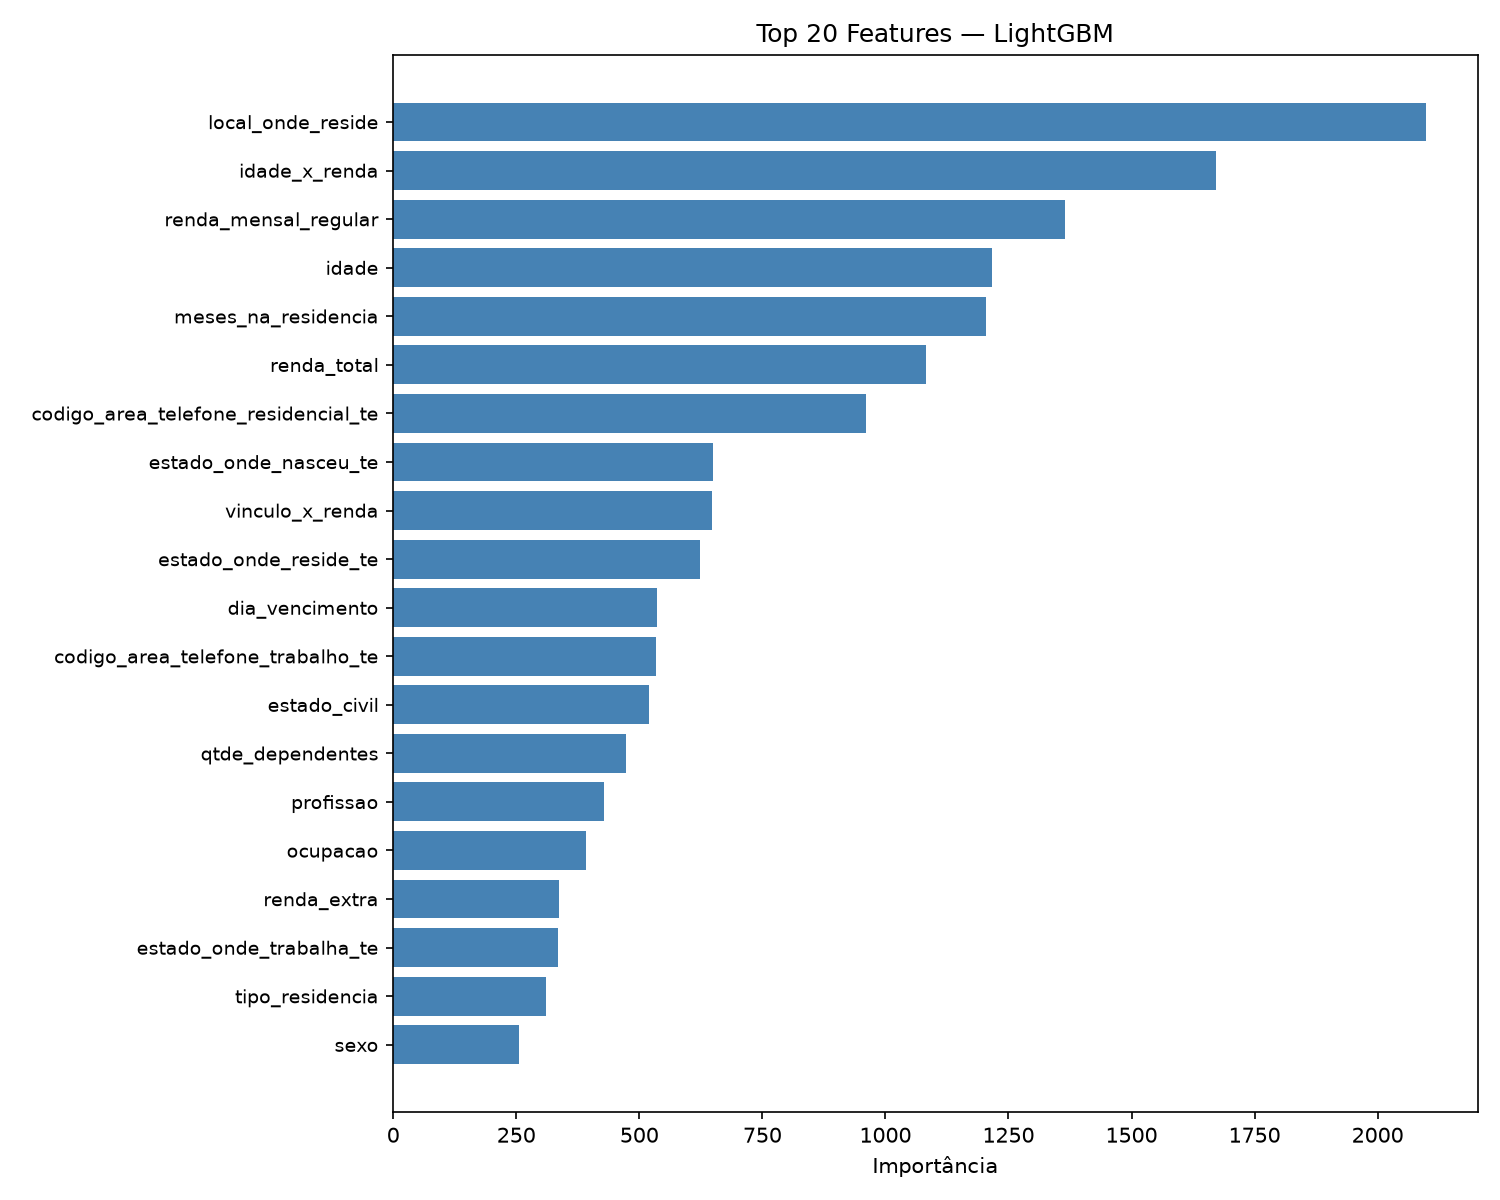
\includegraphics[width=1.0\textwidth]{feature_importance.png}
  \caption{Top 20 \textit{features} por importância no LightGBM otimizado.}
  \label{fig:importance}
\end{figure}

\section{Conclusões}

\begin{enumerate}[leftmargin=2em]
  \item \textbf{Gradient boosting}~\cite{ref:friedman} (LightGBM, XGBoost, CatBoost) superou consistentemente modelos lineares e redes neurais em dados tabulares com sinal fraco.

  \item \textbf{Ensembles} por média de probabilidades e blend multi-seed melhoraram a estabilidade das previsões.

  \item \textbf{Target encoding}~\cite{ref:micci} é poderoso para categóricas de alta cardinalidade, mas deve ser restrito a variáveis onde demonstra consistência entre validação e teste real. O uso indiscriminado causa \textit{data leakage}, como verificado experimentalmente.

  \item \textbf{Mais otimização nem sempre é melhor:} buscas mais longas de hiperparâmetros geraram overfitting ao processo de validação, resultando em scores piores no Kaggle. Isso reforça a importância de validações simples e robustas~\cite{ref:hastie}.

  \item \textbf{O teto de desempenho} é determinado pela qualidade das \textit{features}, não pela sofisticação dos modelos. Múltiplas abordagens diferentes convergiram para a mesma faixa de 0,60--0,61, indicando que o sinal preditivo disponível nos dados é intrinsecamente limitado.
\end{enumerate}

\newpage
\begin{thebibliography}{99}
\addcontentsline{toc}{section}{Referências}

\bibitem{ref:sklearn}
Pedregosa, F. et al. Scikit-learn: Machine Learning in Python. \textit{Journal of Machine Learning Research}, v.~12, p.~2825--2830, 2011.

\bibitem{ref:lgbm}
Ke, G. et al. LightGBM: A Highly Efficient Gradient Boosting Decision Tree. \textit{Advances in Neural Information Processing Systems (NeurIPS)}, v.~30, 2017.

\bibitem{ref:xgb}
Chen, T.; Guestrin, C. XGBoost: A Scalable Tree Boosting System. \textit{Proceedings of the 22nd ACM SIGKDD}, p.~785--794, 2016.

\bibitem{ref:catboost}
Prokhorenkova, L. et al. CatBoost: unbiased boosting with categorical features. \textit{Advances in Neural Information Processing Systems (NeurIPS)}, v.~31, 2018.

\bibitem{ref:optuna}
Akiba, T. et al. Optuna: A Next-generation Hyperparameter Optimization Framework. \textit{Proceedings of the 25th ACM SIGKDD}, p.~2623--2631, 2019.

\bibitem{ref:friedman}
Friedman, J. H. Greedy Function Approximation: A Gradient Boosting Machine. \textit{Annals of Statistics}, v.~29, n.~5, p.~1189--1232, 2001.

\bibitem{ref:breiman}
Breiman, L. Random Forests. \textit{Machine Learning}, v.~45, n.~1, p.~5--32, 2001.

\bibitem{ref:micci}
Micci-Barreca, D. A Preprocessing Scheme for High-Cardinality Categorical Attributes in Classification and Prediction Problems. \textit{ACM SIGKDD Explorations Newsletter}, v.~3, n.~1, p.~27--32, 2001.

\bibitem{ref:hastie}
Hastie, T.; Tibshirani, R.; Friedman, J. \textit{The Elements of Statistical Learning}. 2.~ed. New York: Springer, 2009.

\bibitem{ref:pandas}
McKinney, W. Data Structures for Statistical Computing in Python. \textit{Proceedings of the 9th Python in Science Conference}, p.~56--61, 2010.

\end{thebibliography}

\end{document}